
\subsubsection{thor と optparse のコードの比較}
hikiutilsのコマンドライン解析ツールをoptparseからthorに換えることでコマンドの書き換えを行うことができた.
また,thorで書かれたhikiutilsはoptparseで書かれたものよりもコードが短くなり,コマンドの解析も簡単に行えることができた.
ここではthorとoptparseのコードを比較しthorの良さを確認する.

\paragraph{Thorとoptparseとは}
\paragraph{Thorとは}
Thorとは,コマンドラインツールの作成を支援するライブラリのことである.
gitやbundlerのようにサブコマンドを含むコマンドラインツールを簡単に作成することができる[4].

Thorの基本的な流れとしては
\begin{enumerate}
\item Thorを継承したクラスのパブリックメソッドがコマンドになる
\item クラス.start(ARGV)でコマンドラインの処理をスタートする
\end{enumerate}
という流れである[4].

startに渡す引数が空の場合,Thorはクラスのヘルプリストを出力する.
また,Thorはサブコマンドやサブサブコマンドも作ることができる.

\paragraph{optparseとは}
optparseモジュールとは,getoptよりも簡便で,柔軟性に富み,かつ強力なコマンドライン解析ライブラリである.
optparseでは,より宣言的なスタイルのコマンドライン解析手法,すなわちOptionParserのインスタンスでコマンドラインを解析するという手法をとっている.
これを使うと,GNU/POSIX構文でオプションを指定できるだけでなく,使用法やヘルプメッセージの生成も行える[5].

利用頻度はあまり高くないが古くから開発され,使用例が広く紹介されている.

optparseの基本的な流れとしては
\begin{enumerate}
\item OptionParserオブジェクトoptを生成する
\item オプションを取り扱うブロックをopt.onに登録する
\item opt.parse(ARGV)でコマンドラインを実際にparseする
\end{enumerate}
という流れである.

OptionParserはコマンドラインのオプション取り扱うためのクラスであるためオブジェクトoptを生成されopt.onにコマンドを登録することができる.
しかし,OptionParser\#onにはコマンドが登録されているだけであるため,OptionParser\#parseが呼ばれた時,コマンドラインにオプションが指定されていれば実行される.
optparseにはデフォルトとして--helpと--versionオプションを認識する[6].

\paragraph{コードの解説}
\paragraph{Thorの定義}
\verb|{{attach_view(hikiutils_yamane.003.jpg)}}|
Thorのinitializeの定義のされ方
\begin{enumerate}
\item Hikithor::CLI.start(ARGV)が呼ばれる
\item initializeメソッドが呼ばれる
\item これではThorのinitializeメソッドが呼ばれない
\item superを書くことでThorのinitializeメソッドが呼ばれる
\end{enumerate}
optparseではrequireでoptparseを呼ばれoptparseのinitializeを定義する必要はないが,Thorはinitializeを定義する必要がある.
Thorの定義方法はrequireでThorを呼びCLIクラスで継承し,initializeメソッドにsuperを書くことでThorのinitializeが呼ばれる.
initializeメソッド内ではThorの初期設定がされていないため,スーパークラスのメソッドを読み出してくれるsuperを書き加えることで図のようにinitializeメソッドでThorのinitilalizeメソッドが
呼ばれて定義される.

\paragraph{実際のコード}\begin{lstlisting}[style=customRuby]
# -*- coding: utf-8 -*-                                                         
require 'thor'
require 'kconv'
require 'hikidoc'
require 'erb'
require "hikiutils/version"
require "hikiutils/tmarshal"
require "hikiutils/infodb"
require 'systemu'
require 'fileutils'
require 'yaml'
require 'pp'

module Hikithor

  DATA_FILE=File.join(ENV['HOME'],'.hikirc')
  attr_accessor :src, :target, :editor_command, :browser, :data_name, :l_dir

  class CLI < Thor
   def initialize(*args)
      super
      @data_name=['nick_name','local_dir','local_uri','global_dir','global_uri']
      data_path = File.join(ENV['HOME'], '.hikirc')
      DataFiles.prepare(data_path)

      file = File.open(DATA_FILE,'r')
      @src = YAML.load(file.read)
      file.close
      @target = @src[:target]
      @l_dir=@src[:srcs][@target][:local_dir]
      browser = @src[:browser]
      @browser = (browser==nil) ? 'firefox' : browser
      p editor_command = @src[:editor_command]
      @editor_command = (editor_command==nil) ? 'open -a mi' : editor_command
   end
\end{lstlisting}
\paragraph{hikiutilsの実行}\begin{itemize}
\item Thor
\end{itemize}
\begin{figure}[htbp]\begin{center}
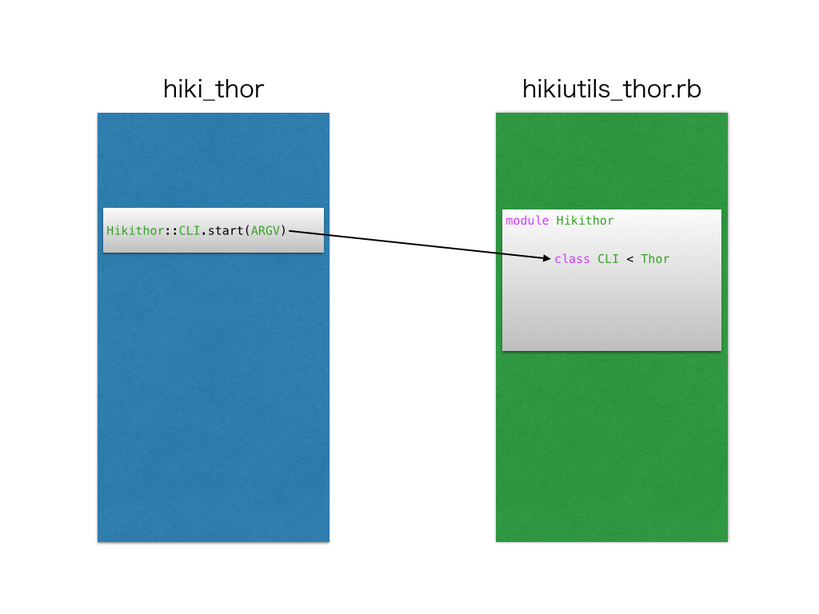
\includegraphics[width=6cm,bb=0 0 442 500]{../figs/./hikiutils_yamane.004.jpg}
\caption{}
\label{default}\end{center}\end{figure}\begin{enumerate}
\item hiki\_thorのHikithor::CLI.start(ARGV)でhikiutils\_thor.rbのCLIクラスを呼ぶ
\end{enumerate}\begin{enumerate}
\item hikiutils\_thor.rbのCLIクラスのメソッドを順に実行していく
\end{enumerate}\begin{itemize}
\item optparse
\end{itemize}
\begin{figure}[htbp]\begin{center}
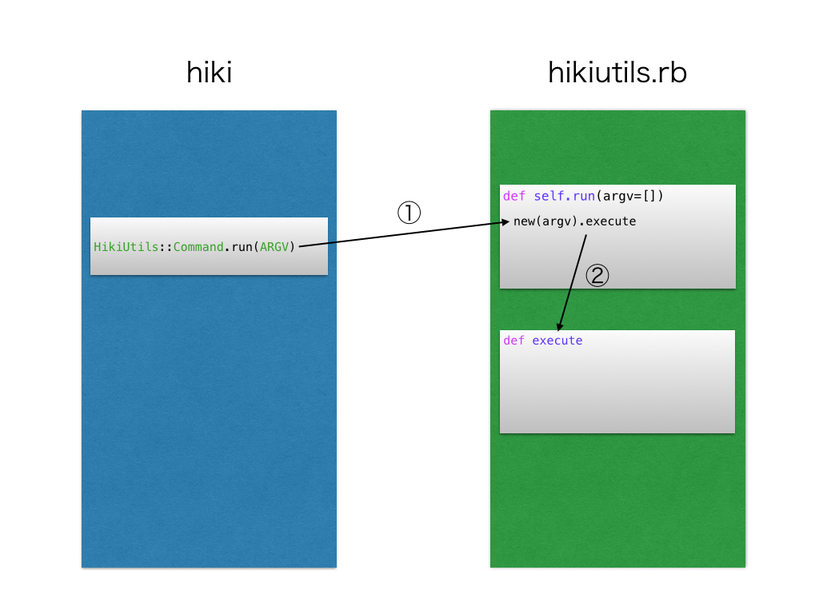
\includegraphics[width=6cm,bb=0 0 442 500]{../figs/./hikiutils_yamane.001.jpg}
\caption{}
\label{default}\end{center}\end{figure}\begin{enumerate}
\item HikiのHikiUtils::Command.run(ARGV)でhikiutils.rbのrunメソッドを呼ぶ
\item new(argv).executeでexecuteメソッドが実行される
\end{enumerate}
このようにoptparseでは実行を行うためのメソッドが必要であるが,Thorではクラスのメソッドを順に実行していくため
runメソッドとexecuteメソッドは必要ない.

\paragraph{実際のコード}\begin{itemize}
\item Thor
\end{itemize}\begin{lstlisting}[style=customRuby]
#!/usr/bin/env ruby                                                             

require "hikiutils_thor"

Hikithor::CLI.start(ARGV)
\end{lstlisting}\begin{lstlisting}[style=customRuby]
# -*- coding: utf-8 -*-                                                         
require 'thor'
require 'kconv'
require 'hikidoc'
require 'erb'
require "hikiutils/version"
require "hikiutils/tmarshal"
require "hikiutils/infodb"
require 'systemu'
require 'fileutils'
require 'yaml'
require 'pp'

module Hikithor

  DATA_FILE=File.join(ENV['HOME'],'.hikirc')
  attr_accessor :src, :target, :editor_command, :browser, :data_name, :l_dir

  class CLI < Thor
   def initialize(*args)
      super
      @data_name=['nick_name','local_dir','local_uri','global_dir','global_uri']
      data_path = File.join(ENV['HOME'], '.hikirc')
      DataFiles.prepare(data_path)

      file = File.open(DATA_FILE,'r')
      @src = YAML.load(file.read)
      file.close
      @target = @src[:target]
      @l_dir=@src[:srcs][@target][:local_dir]
      browser = @src[:browser]
      @browser = (browser==nil) ? 'firefox' : browser

\end{lstlisting}\begin{itemize}
\item optparse
\end{itemize}\begin{lstlisting}[style=customRuby]
#!/usr/bin/env ruby                                                             

require "hikiutils"

HikiUtils::Command.run(ARGV)
\end{lstlisting}\begin{lstlisting}[style=customRuby]
    def self.run(argv=[])
      print "hikiutils: provide utilities for helping hiki editing.\n"
      new(argv).execute
    end

    def execute
      @argv << '--help' if @argv.size==0
      command_parser = OptionParser.new do |opt|
        opt.on('-v', '--version','show program Version.') { |v|
          opt.version = HikiUtils::VERSION
          puts opt.ver
        }
        opt.on('-s', '--show','show sources') {show_sources}
        opt.on('-a', '--add','add sources info') {add_sources }
        opt.on('-t', '--target VAL','set target id') {|val| set_target(val) }
        opt.on('-e', '--edit FILE','open file') {|file| edit_file(file) }
        opt.on('-l', '--list [FILE]','list files') {|file| list_files(file) }
        opt.on('-u', '--update FILE','update file') {|file| update_file(file) }
        opt.on('-r', '--rsync','rsync files') {rsync_files}
        opt.on('--database FILE','read database file') {|file| db_file(file)}
        opt.on('--display FILE','display converted hikifile') {|file| display(f\
ile)}
        opt.on('-c', '--checkdb','check database file') {check_db}
        opt.on('--remove FILE','remove file') {|file| remove_file(file)}
        opt.on('--move FILES','move file1,file2',Array) {|files| move_file(file\
s)}
        opt.on('--euc FILE','translate file to euc') {|file| euc_file(file) }
        opt.on('--initialize','initialize source directory') {dir_init() }
      end
      begin
        command_parser.parse!(@argv)
      rescue=> eval
        p eval
      end
      dump_sources
      exit
    end  
\end{lstlisting}
\paragraph{コマンドの表示と処理}\begin{itemize}
\item Thor
\end{itemize}
\begin{figure}[htbp]\begin{center}
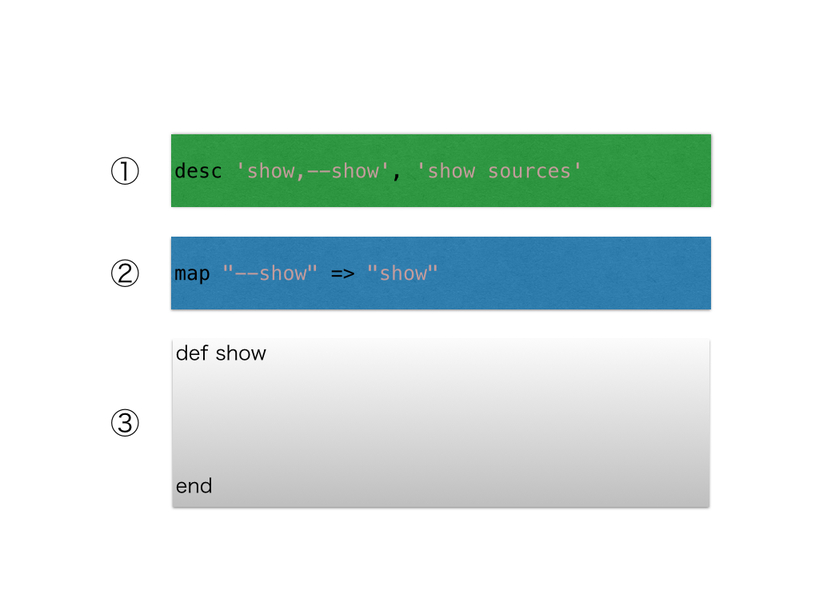
\includegraphics[width=6cm,bb=0 0 442 500]{../figs/./hikiutils_yamane.002.jpg}
\caption{}
\label{default}\end{center}\end{figure}\begin{enumerate}
\item コマンド名,コマンドの説明を一覧に表示させる
\item パブリックメソッドのコマンドを別のコマンド名でも実行できるようにする
\item コマンドの命令の実行コード
\end{enumerate}
Thorではdescで一覧を表示させるコマンド名,コマンドの説明を登録する.しかし,ここで記述したコマンドは一覧で表示させるものであり,実行されることはないので実際のコマンドと対応させる必要がある.
Thorでは処理実行を行うメソッドがコマンドとなる.しかし,それではコマンド名は1つしか使うことができない.
ここで用いるものがmapである.mapを使うことで別のコマンドを指定することができる.
\begin{itemize}
\item optparse
\end{itemize}
\begin{figure}[htbp]\begin{center}
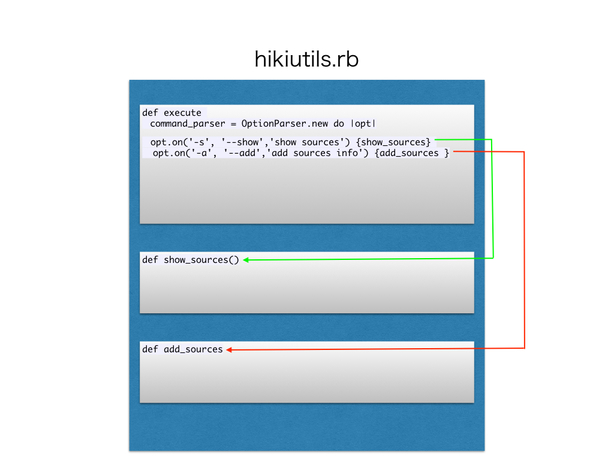
\includegraphics[width=6cm,bb=0 0 442 500]{../figs/./hikiutils_yamane.005.jpg}
\caption{}
\label{default}\end{center}\end{figure}\begin{enumerate}
\item OptionParserオブジェクトoptを生成
\item optにコマンドを登録
\item 入力されたコマンドの処理のメソッドへ移動
\end{enumerate}
optparseではOptionParserオブジェクトoptの生成を行い,コマンドをoptに登録することでコマンドを作成することができる.しかし,これはコマンドを登録しているだけで
コマンドの一覧ではこれを表示することができるがコマンドの実行を行うためには実行を行うためのメソッドを作成する必要がある.optparseでのコマンドの実行はoptで登録された
コマンドが入力されることでそれぞれのコマンドの処理を行うメソッドに移動し処理を行う.しかし,このコマンド登録は-を付けたコマンドした登録ができなく,-なしのコマンド登録は
また別のやり方でやらなくてはいけない.
以上より,Thorではコマンドの指定と処理にはdesc,map,処理メソッドだけで済むが,optparseではコマンドを登録するためのメソッドと処理メソッドが必要になってくる.
また,コマンドはThorでは処理メソッドがコマンド名になるが,optparseではコマンドを登録するための処理も必要となってくる.

\paragraph{実際のコード}\begin{itemize}
\item Thor
\end{itemize}\begin{lstlisting}[style=customRuby]
    desc 'show,--show', 'show sources'
    map "--show" => "show"
    def show
      printf("target_no:%i\n",@src[:target])
      printf("editor_command:%s\n",@src[:editor_command])
      @i_size,@n_size,@l_size,@g_size=3,5,30,15 #i,g_size are fixed             
      n_l,l_l=0,0
      @src[:srcs].each_with_index{|src,i|
        n_l =(n_l= src[:nick_name].length)>@n_size? n_l:@n_size
        l_l =(l_l= src[:local_dir].length)>@l_size? l_l:@l_size
      }
      @n_size,@l_size=n_l,l_l
      command = Command.new
      header = command.display_format('id','name','local directory','global uri',@i_size,@n_size,@l_size,@g_size)

      puts header
      puts '-' * header.size

      @src[:srcs].each_with_index{|src,i|
        target = i==@src[:target] ? '*':' '
        id = target+i.to_s
        name=src[:nick_name]
        local=src[:local_dir]
        global=src[:global_uri]
        puts command.display_format(id,name,local,global,@i_size,@n_size,@l_size,@g_size)
      }
    end
\end{lstlisting}\begin{itemize}
\item optparse
\end{itemize}\begin{lstlisting}[style=customRuby]
    def execute
      @argv << '--help' if @argv.size==0
      command_parser = OptionParser.new do |opt|
        opt.on('-v', '--version','show program Version.') { |v|
          opt.version = HikiUtils::VERSION
          puts opt.ver
        }
        opt.on('-s', '--show','show sources') {show_sources}
        opt.on('-a', '--add','add sources info') {add_sources }
        opt.on('-t', '--target VAL','set target id') {|val| set_target(val)}
        opt.on('-e', '--edit FILE','open file') {|file| edit_file(file) }
        opt.on('-l', '--list [FILE]','list files') {|file| list_files(file)}
        opt.on('-u', '--update FILE','update file') {|file| update_file(file) }
        opt.on('-r', '--rsync','rsync files') {rsync_files}
        opt.on('--database FILE','read database file') {|file| db_file(file)}
        opt.on('--display FILE','display converted hikifile') {|file| display(file)}
        opt.on('-c', '--checkdb','check database file') {check_db}
        opt.on('--remove FILE','remove file') {|file| remove_file(file)}
        opt.on('--move FILES','move file1,file2',Array) {|files| move_file(files)}
        opt.on('--euc FILE','translate file to euc') {|file| euc_file(file)}
        opt.on('--initialize','initialize source directory') {dir_init() }
      end
      begin
        command_parser.parse!(@argv)
      rescue=> eval
        p eval
      end
      dump_sources
      exit
    end    
    
    def show_sources()
      printf("target_no:%i\n",@src[:target])
      printf("editor_command:%s\n",@src[:editor_command])
      check_display_size()
      header = display_format('id','name','local directory','global uri')

      puts header
      puts '-' * header.size

      @src[:srcs].each_with_index{|src,i|
        target = i==@src[:target] ? '*':' '
        id = target+i.to_s
        name=src[:nick_name]
        local=src[:local_dir]
        global=src[:global_uri]
        puts display_format(id,name,local,global)
      }
    end

    def add_sources
      cont = {}
      @data_name.each{|name|
        printf("%s ? ", name)
        tmp = gets.chomp
        cont[name.to_sym] = tmp
      }
      @src[:srcs] << cont
      show_sources
    end
\end{lstlisting}
コードからもThorのほうが短くなっていることが分かる.
よって,Thorとoptparseでのコードの違いは以上の部分になるが全体的にもThorのほうがコードが短くなり,
コマンドの定義も簡単に行うことができる.また,コマンドを簡単に定義できることで書き換えもすぐ行うことが
できるので,より直感的なコマンドに実装することも可能となった.

